
\chapter{Compression systems}
\section{Introduction and different types of compressors}
\subsection{Purpose and compressor types}
Turbocompressors are systems used to convert shaft mechanical energy into fluid pressure and kinetic energy. The fluid can be air and other special gases like nitrogen or whatever. When the inlet pressure is lower than atmospheric one and that output pressure is the atmospheric pressure we speak of \textbf{vacuum pump} and when the exhaust pressure is low with one stage of blades it is a \textbf{fan} or a \textbf{ventilator}.

\subsubsection{Reciprocating / piston compressors}
\wrapfig{9}{l}{3}{0.2}{ch5/1}
There exists two big families of compressors: the volumetric compressors and the turbocompressors. The first family consists in machines that compress by decreasing the gas volume (reciprocating compressors for ex) and the second compresses through a rotor that redirects the flow. A problem of the volumetric compressors is the lack of continuity due to the injection, we need a tank. We also need lubricant where metal-metal contact happens. Leakage around the piston is also a problem and the friction increases the need for maintenance. 
Discharge pressures can go from very low pressures to very high (180 MPa)

\subsubsection{Rotary vane compressors}
\wrapfig{8}{r}{3}{0.3}{ch5/2}
Rotary compressors are composed of a rotor with blades inserted in radial slots, placed offset in a larger circular (or complex shape) housing. When the machine rotates, the blades are moving in the slots so that the volume which confine the air decreases with the angle. This is similar to the piston compressor but is quiter and can go up to 1.3 MPa in one stage. Its efficiency is around 90\% .

\subsubsection{Roots compressors and rotary screw compressors} 
\minifig{ch5/3}{ch5/4}{0.3}{0.3}{0.4}{0.4}

Roots compressors pressure ratio and mass flow rate are very low but works very smoothly (low vibrations and noise), \autoref{ch5/3}. Rotary screw compressors are composed of two meshed rotating positive-displacement helical screws in order to force the fluid in smaller spaces. These are used for continuous operation, has a power between 2.2 up to 890 kW and pressures up to 8.3 MPa. Types: oil flooded, water flooded and dry. The longer the screw the higher the compression ratio. 

\subsubsection{Turbocompressors}
\wrapfig{8}{l}{6}{0.3}{ch5/5}
They are similar to the pumps, centrifugal compressor composed of a bladed rotor that gives kinetic energy to the fluid and then it is converted into pressure in the divergent duct. They can have very high exhaust pressures (up to 69 MPa with multistage). Almost no metal-metal contact so the maintenance request is very low. 

\ \\
For high flow rate and compact design we use the axial flow compressors (\autoref{ch5/5}). They are almost always composed of multistage, the cross sectional area decreases at each stage, one rotor followed by one stator. 

\subsection{Use of different compressor types}
They differs from diverse parameters: 

\begin{itemize}
\item[•] Mass flow rate: huge for axial turbocompressors, large for centrifugal turbo and rather small for all other \\
\item[•] Maximum ratio per stage: large for centrifugal turbo, medium for piston compressors and very small for axial turbo, but axial turbo is the only one where it is easy to put series of stages and reach very high ratios
\item[•] Poor air (no pollutants): axial and centrifugal turbo are very good for that, piston and rotary vane types are very poor because of the lubricant. 
\end{itemize}

\section{Fundamental equations for gas compression systems}
\subsection{Definitions and nomenclature}
\subsubsection{Admission and exhaust pressure}
The volume from which we take air is called \textbf{aspiration medium} or \textbf{aspiration environment} and the pressure there $p_0$ is the \textbf{aspiration pressure}. Similarly for the exit we have the \textbf{exhaust} medium, environment and pressure $p_1$. The losses in the piping are not negligible. 

\subsubsection{Compressor pressure ratio}
It is defined in terms of the \textbf{total} pressure, because in the theorem of kinetic energy the velocity intervenes: 

\begin{equation}
\pi _c = \frac{p_{t, out}}{p_{t, in}}
\end{equation}

\subsubsection{Flow rate}
Mass flow rate (kg/s) are used instead of volumetric flow rate ($m^3$/s) because if we use the second we have to specify the conditions at the exhaust and the intrance (change in density), while mass flow rate stays constant (very small leak losses).

\subsubsection{Specific energy consumption}
The specific consumption is the ratio between the driving power and the volumetric flow rate: 

\begin{equation}
SFC = \frac{P_m}{Q_{out}}
\end{equation} 

This is for the manufacturer not for us. For large to medium, water cooled compressors it is about 280-310 J/l and can be 3-5\% higher for air cooled (1\% absorbed by cooling fan). 

\subsection{Fundamental thermodynamics law}
\subsubsection{Introduction}
We will only consider steady state, so not the transients (accelerations and decelarations of the machine) and variations of aspiration and exhaust conditions. 

\minifig{ch5/6}{ch5/7}{0.4}{0.4}{0.4}{0.4}

We will apply the first principle and second principle of thermodynamics and also the kinetic energy equation on a given mass of gas contained initially between the volume $A_0, A_1$ and a period later so at $t+\Delta t$ between $A_0', A_1'$ as represented on the figures for the reciprocating and turbo compressors. For the piston, the time interval corresponds to a piston period while for turbocompressors it is arbitrary. The mass of air between $A_0$ and $A_0'$ is always the same as the one contained in $A_1$ and $A_1'$, the mass between $A_0'$ and $A_1$ is also always constant and thermodynamic variables are all the same at $t$ and $t+ \Delta t$.

\subsubsection{Use of the energy equation}
He skipped all the equations before. The energy equation is: 

\begin{equation}
q + p_0 \nu_0 - p_1 \nu _1 + w_i = u_1 - u_0 + \frac{v_1 ^2 - v_0^2}{2} + g(z_1-z_0)
\end{equation}

Combining pressure and $u$ terms to get $h$ and neglecting the level difference $\Delta z$: 

\begin{equation}
q + w_i = h_1 - h_0  \qquad \Rightarrow (q= 0) \ w_i = \Delta h = c_p \Delta T\qquad  \Leftrightarrow P_i = \dot{m} c_p \Delta T
\end{equation}

\subsubsection{Second fundamental thermodynamics law}
We have that: 

\begin{equation}
ds = \delta q/T + ds_{irr} \quad \Rightarrow Tds = dh - \nu dp = \delta q + ds_{irr} \quad \Rightarrow h_1 - h_0 - \int _0 ^1 \nu dp = q + \int _0 ^1 Tds_{irr}
\end{equation}

We see that the integration gives something similar to what we had before but with an additional irreversible term. 

\subsubsection{Kinetic energy equation}
By combining the two last equations we got: 

\begin{equation}
w_i = \int _0 ^1 \nu dp + \int _0 ^1 Tds_{irr}
\end{equation}

We see that the work provided by the piston or the rotor is used to increase the pressure and to compensate the losses due to irreversibility. 

\subsubsection{Total system of equations}
\theor{
Total energy equation: 
\begin{equation}
q + w_i = h_1 -h_2 
\end{equation}

Kinetic energy equation: 

\begin{equation}
w_i = \int _0 ^1 \nu dp + \int _0 ^1 Tds_{irr}
\end{equation}

Global thermodynamic equation

\begin{equation}
\int _0^1 Tds = h_1 - h_0 - \int _0 ^1 \nu dp = q + \int _0 ^1 Tds_{irr}
\end{equation}
}\ \\

\section{Compression of perfect gases}
\subsection{Reference compression modes}
Since it is impossible to model the real compression mode because of the irreversibilities. We will study 3 types of compression to see the effects of some parameters: 

\begin{itemize}
\item[•] Reversible isothermal compression 
\item[•] Reversible adiabatic compression (isentropic compression)
\item[•] Polytropic compression
\end{itemize}

The fluid is considered to be a perfect gas with $c_p = cst$.

\subsection{Reversible internal compression}
\subsubsection{Internal work and internal power}
Assuming the compressor to be highly cooled, we can assume isothermal process. We neglect irreversibilities and thus the energy equation of previous section becomes: 

\begin{equation}
w_{it} + q = h_1 -h_0 = c_p\Delta T = 0 \qquad w_{it} = -q
\end{equation}

The internal work is thus equal to the heat to be extracted from the compressed gas to keep the temperature constant. The kinetic energy equation gives: 

\begin{equation}
w_{it} = \int _0 ^1 \nu dp = RT_0 \ln \pi _c \qquad \Rightarrow P_{it} = \dot{m} rT_0 \ln \pi _c
\end{equation}

where we used the perfect gas relation $\nu = rT_0/p$. We deduce that indeed higher pressure ratios require higher works, but also higher temperatures require higher work (not the same in winter and summer). 

\subsubsection{Presentation on the entropy diagram}
\wrapfig{8}{l}{4.5}{0.3}{ch5/8}
Since the inlet conditions $p_0,T_0$ are known, we have the aspiration point on the T-S diagram. To obtain the exhaust conditions it is sufficient to keep the temperature constant and to jump on $p_1$ curve (reversible so straight line).  From the fundamental second law: 

\begin{equation}
q = \int _0 ^1 Tds = T_0 (s_{1t}- s_0) = \overline{0 - 1_t}
\end{equation}

We see that the heat extracted corresponds to the area corresponding to the projection of the $\overline{0-1_t}$ curve on s axis. Covered anticlockwise it is the negative direction so we have the heat and clockwise direction corresponds to $w_i$: 

\begin{equation}
w_i = \overline{1_t - 0}
\end{equation} 

\subsection{Isentropic compression}
This time we consider adiabatic and reversible compression $q=0 = \int Tds_{irr}$. The energy equation gives: 

\begin{equation}
w_{is} = h_1 - h_0 = c_p T_0 \left(\frac{T_{1s}}{T_0} - 1\right) = c_p T_0 \left(\pi ^{\frac{\chi - 1}{\chi}} _c- 1\right)
\end{equation}

where the compression ratio comes from isentropic law. On the other hand: 

\begin{equation}
r = c_p - c_v = c_p \left( 1 - \frac{1}{\chi} \right) \qquad \Rightarrow c_p = \frac{\chi}{\chi -1} r
\end{equation}

Injecting this in previous expression: 

\begin{equation}
w_{is} = \frac{\chi}{\chi -1} r T_0 \left(\pi ^{\frac{\chi - 1}{\chi}} _c- 1\right)
\end{equation}

Again work is increasing with compression ratio and it is shown with an example in the syllabus that it is higher than the iso-T case! 

\subsubsection{Presentation on the entropy diagram}
\wrapfig{8}{r}{4.5}{0.3}{ch5/9}
Consider an additional point which is $1_t$ for this diagram, the point $1_s$ is obtained with the isentropic evolution. Since temperatures are the same at $1_t$ and $0$, $h_{1s} - h_0 = h_{1s} - h_{1t}$. If we imagine an evolution between $1_t and 1_s$ and apply the second fundamental relation: 

\begin{equation}
\int _{1t} ^{1s} = h_{1s} - h_{1t} + \cancel{\int \nu dp} = w_{is} = \overline{1_t - 1_s}
\end{equation}

That projection area is larger than the iso-T case as deduced. 

\subsection{Polytropic compression}
\subsubsection{Definition}
The evolution that matches the best the real life evolution is the polytropic evolution. The final point ($p_1,T_1$) is the same as the real life while not in iso-T and iso-S. The evolution respects: 

\begin{equation}
p_1\nu_1^" = p_2\nu _2^"
\end{equation}

This injected in the perfect gas law: 

\begin{equation}
\frac{T_1}{T_0} = \left( \frac{p_1}{p_0}\right)^{\frac{n-1}{n}} \qquad T_1\nu_1^{n-1} = T_0\nu_0^{n-1}
\end{equation}

where $n$ is the polytopric exponent, similar to the $\gamma$ of the isentropic evolution. 

\subsubsection{Experimental determination of the polytropic exponent}
It is easily found as follows: 

\begin{equation}
\frac{T_1}{T_0} = \left( \frac{p_1}{p_0}\right)^{\frac{n-1}{n}} \Leftrightarrow \frac{n}{n-1} = \frac{\ln \frac{T_1}{T_0}}{\ln \frac{p_1}{p_0}} \qquad \Rightarrow n = \frac{\ln \frac{p_1}{p_0}}{\ln \frac{p_1}{p_0} - \ln \frac{T_1}{T_0}}
\end{equation}

\subsubsection{Internal work and internal power}
Again, we can neglet irreversibility, and using the kinetic energy equation we can get (no development given): 

\begin{equation}
w_{ip} = \frac{n}{n-1}rT_0\left( \pi _c ^{\frac{n-1}{n}} -1 \right)
\end{equation}

\subsubsection{Presentation on the entropy diagram}
A distinction has to be made between cooked systems and adiabatic systems

\wrapfig{6}{l}{4.5}{0.3}{ch5/10}
\paragraph{Cooled compression}
In practice, the cooling is larger than the irreversible effect so that the thermodynamic relation tells that entropy decreases: 

\begin{equation}
\int _0^1 Tds = q + \int Tds _{irr} \qquad \Leftrightarrow \overline{1-0} = -q
\end{equation}

We see that the projection area under the curve 1-0 (positive direction) corresponds to the heat to be extracted. On the other hand, the energy equation tells that: 

\begin{equation}
w_i + q = h_1 - h_0 = h_1 - h_{1t} = \overline{1_t - 1} \qquad \Leftrightarrow w_{ip} = \overline{1_t -1 -0}
\end{equation}

\wrapfig{6}{l}{4.5}{0.3}{ch5/11}
\paragraph{Adiabatic compression}
A real compression is non-reversible and adiabatic. The polytropic compression that we use is reversible but not adiabatic anymore. Indeed, the real point on the graph would be not reachable in that case since reversible + adiabatic = isentropic. In fact, the effects of the non reversibilities are replace by an addition of heat: 

\begin{equation}
w_i + q = h_1 - h_0 = h_1 - h_{1t} = \overline{1_t - 1} \qquad \int _0^1 Tds = q = \overline{0-1}
\end{equation}

Substraction of the two projection surfaces gives: 

\begin{equation}
w_{ip} = \overline{1_t - 1 - 0}
\end{equation}

\subsection{Cooled compressors - refrigerated compression}
\subsubsection{Application and presentation on the entropy diagram}
Piston compressors are cooled because the lubricant looses its properties at very high temperature and then can pollute the air. \\

\wrapfig{6}{r}{4.5}{0.3}{ch5/12}
Take for example a 3 stage compressor. The initial point in the first stage is noted $0^1$ and the compression goes to point $1^1$. Then using an intermediate heat exchanger, the fluid is cooled down to $0^2$. $T_2>T_1$ because we try to keep the dimensions and frictions in the exchanger acceptable. Large pressure losses occur in the exchanger so $p_0^2 < p_1^1$. Then the same for the other stages. 

\subsubsection{Determination of partial compressor pressure ratios}
\wrapfig{6}{l}{4.5}{0.3}{ch5/13}
We will try to determine the best inter pressure ratio (minimum $w_i$) for a multi-stage compressor. For this consider the following assumptions: 

\begin{itemize}
\item[•] The compression in each stage follows a polytropic evolution with the same coefficient $n$ that depends on the level of cooling that one applies. Same cooling is used so. 
\item[•] The pressure losses in the coolers are neglected and they bring the fluid to the initial temperature $T_0$
\end{itemize}

\ \\
Consider $k$ stages and $k$ different pressure $p^1, \dots, p^{k-1}$. The starting pressure is $p_0^1$ and the exhaust $p_1^k$. For each stage $i$ we know the internal work expression and we can sum up over $k$ stages: 

\begin{equation}
w_{ip}^i = \frac{n}{n-1}rT_0\left[ \left(\frac{p^i}{p^{i-1}} \right) ^{\frac{n-1}{n}} -1 \right] \qquad \Rightarrow \sum _{i=1}^k w_{ip}^i = \frac{n}{n-1}rT_0\left[ \left(\sum _{i=1} ^k\frac{p^i}{p^{i-1}} \right) ^{\frac{n-1}{n}} -k \right]
\end{equation}

We see that the minimum work is obtained when the sum of pressure ratios is minimum. We can see that the product of these terms is constant: 

\begin{equation}
\Pi _{i=1}^k \left(\frac{p_i}{p_{i-1}} \right)^{\frac{n}{n-1}} = \left(\frac{p_1^1}{p_0^1} \dots \frac{p_1^k}{p_0^k} \right)^{\frac{n}{n-1}} = \pi _c^{\frac{n}{n-1}}
\end{equation}

This means that the sum is minimal when all pressure ratios are equal. In that case one can find that the best stage pressure ratio is: 

\begin{equation}
\frac{p_1^i}{p_0^i} = \sqrt[k]{\pi _c}
\end{equation} 

Don't forget that if we considered the pressure and temperature losses in the coolers, this value could be slightly different. 

\subsection{Standard working conditions}
The comparison of different compressors can be very difficult if standard conditions are not defined, since the work is dependent on the inlet temperature, the mass flow rate depends on the inlet density of the gas $\rho$, ... We impose the manufacturer to give data considering standard inlet conditions, at sea level: 

\begin{equation}
T_a = 15\degres C = 288 \, K \qquad p_a = 101325\, Pa
\end{equation}

\section{Efficiency definitions}
\subsection{Global efficiency of a compressor}
\subsubsection{Definition}
The mechanical power $P_m$ is the power applied on the compressor shaft via a driving machine. This is not totally transferred to the fluid, there are mechanical losses in the bearing and the seals for example, but they can occur between the cylinder and the piston or on the rotor of a rotary vane compressor. We can have also a thermodynamic or aerodynamic origin like the friction in the fluid due to the boundary layer, gradients in the thermodynamic variables or a non-perfect cooling system. The \textbf{global efficiency} compares the internal power that would be needed for an ideal compressor without losses and the power really consumed: 

\begin{equation}
\eta = \frac{(P_i)_{id}}{P_m}
\end{equation}

Adapted to an isothermal compressor and an adiabatic compressor, we use the previously computed internal powers: 

\begin{equation}
\eta = \frac{P_{it}}{P_m} \qquad \eta = \frac{P_{is}}{P_m}
\end{equation}

\subsection{The mechanical efficiency and the internal efficiency}
Similarly to what we have done in previous chapters, we can split the global efficiency into internal and mechanical efficiencies to know the part of thermodynamic losses and mechanical losses: 

\begin{equation}
\eta = \frac{(P_i)_{id}}{P_m} = \frac{(P_i)_{id}}{P_i} \frac{P_i}{P_m} = \eta _i \eta _m
\end{equation}

In that case, $P_i$ is the internal power available at the center of the rotor in a turbocompressor or on the piston head in a piston compressor. 

\subsection{Isentropic efficiency}
It is used for adiabatic compressors where the compression is isentropic: 

\begin{equation}
\eta _{is} = \frac{P_{is}}{P_i}
\end{equation}

Using the definition of the internal work we can express it as: 

\begin{equation}
\begin{aligned}
P_{is}= \dot{m} &w_{is} = \dot{m}(h_{is}-h_0) = \dot{m} c_p (T_{is} - T_0)\\
P_{i}= \dot{m} &w_{i} = \dot{m}(h_{1}-h_0) = \dot{m} c_p (T_{1} - T_0)\\
\Rightarrow &\eta _{is}= \frac{T_{is} - T_0}{T_{1} - T_0} = \frac{\pi _c ^{\frac{\gamma -1}{\gamma}} - 1}{\frac{T_1}{T_0} - 1}
\end{aligned}
\end{equation}

\subsection{Polytropic efficiency}
The polytropic efficiency describing better the real compression, the polytropic efficiency will be higher than the others. It can be expressed using the following relations: 

\begin{equation}
\begin{aligned}
P_{pol} = &\dot{m} \frac{n}{n-1}r(T_1 - T_0) \qquad P_i = \dot{m }c_p (T_1 - T_0)\\
\Rightarrow &\eta _{pol} = \frac{n}{n-1}\frac{r}{c_p} = \frac{n}{n -1} \frac{c_p - c_v}{c_p} = \frac{n}{n-1}\frac{\gamma -1}{\gamma}
\end{aligned}
\end{equation}

Using this equation, the polytropic coefficient can be computed if the efficiency is known.

\subsection{Relation between polytropic and isentropic efficiency}
In the case of the isentropic efficiency and the polytropic efficiency we have respectively: 

\begin{equation}
\frac{T_{is}}{T_0} = \pi _c ^{\frac{\gamma-1}{\gamma}} = \theta \qquad \frac{T_{1}}{T_0} = \pi _c ^{\frac{n-1}{n}} = \pi _c ^{\frac{\gamma - 1}{\gamma \eta_{pol}}} =  \theta ^{\frac{1}{\eta_{pol}}}
\end{equation}

This leads when rethinking about the definition of the isentropic efficiency to: 

\begin{equation}
\eta _{is} = \frac{\theta - 1}{\theta ^{\frac{1}{\eta _{pol}}}-1}
\end{equation}

\paragraph{Observations} 

\begin{itemize}
\item[•] The isentropic efficiency depends on the pressure ratio and decreases when the ratio increases
\item[•] The polytropic efficiency does not depend on the pressure ratio and is thus a better parameter to describe aerodynamic properties
\item[•] The polytropic efficiency is higher than the isentropic, and when the pressure ratio decreases the isentropic tends to the polytropic.
\end{itemize}

\section{Reciprocating / Piston compressors}
\subsection{Nomenclature}
\minifig{ch5/14}{ch5/15}{0.6}{0.6}{0.4}{0.4}

These are already known from the course Piston engines. Let's recall that the piston top is not moving in all the cylinder, there is a dead volume called \textbf{clearance volume} on top due to the space taken by the valves. The position of the piston head at top is called \textbf{top dead center} and on bottom, \textbf{bottom dead center}. The \textbf{displacement volume} also called qualifies the volume in which the piston moves and that corresponding distance is called \textbf{stroke}. The \textbf{compression ratio} is expressed in terms of volume: 

\begin{equation}
r = \frac{V_{max}}{V_{min}} = \frac{V_{BDC}}{V_{TDC}}
\end{equation}

\subsection{How it works in theory}
\subsubsection{Theoretical indicator diagram}
\wrapfig{7}{l}{6}{0.3}{ch5/16}
The assumptions we use are that we have a constant rotational speed and steady state conditions, no leak in valves and piston. On the figure is represented an \textbf{indicator diagram}. Let's start at point B where the piston is at BTC. The compression starts (exhaust valve closed) until reaching the exhaust environment pressure on point C. The evolution is supposed to be polytropic with a cooling system. Then the exhaust valve is open and the piston goes to the TDC where the volume is the dead volume, point D. Then the valve is closed and the small air quantity is expanded till reaching the intake environment pressure at point A. The polytropic evolution $n$ coefficient is smaller in expansion due to the reduced mass of air. There the intake valve is open and the air is admitted till reaching the BTC. Then the process repeats.

\subsubsection{Indicated work and power}
\wrapfig{7}{r}{4}{0.3}{ch5/17}
We can express the work in the cylinder using its basic definition of force times a displacement: 

\begin{equation}
\delta W_{p\rightarrow g} = (p-p_a) A\, dx \qquad \Rightarrow W_{ind} = \oint (p-p_a)A\, dx = -\oint p\, dv = \oint v \, dp
\end{equation}

And the power is expressed as: 

\begin{equation}
P_{ind}= \frac{n}{60}\oint v\, dp
\end{equation}

\subsubsection{Theoretical filling coefficient}
During the intake phase, a first expansion has to be made from $p_1$ to $p_0$ and only then the intake begins (this is due to the dead volume). The filling coefficient $x_{th}$ is the ratio between the volume that is effectively intaken by the piston and the total displacement volume: 

\begin{equation}
x_{th} = \frac{v_{AB}}{v_1}
\end{equation}

Let's try to express this in terms of pressure. We know from the idicator diagram that $v_{AB} = v_c + v_1 - v_{aA}$ and from the polytropic law that $p_1 v_c^n = p_0 v_{aA}^n \Rightarrow v_{aA} = v_c\pi _c^{1/n}$ so that: 

\begin{equation}
x_{th} = 1 - \alpha \left( \pi _c^{\frac{1}{n}} -1 \right) \qquad \alpha = \frac{v_c}{v_1}
\end{equation}

\subsubsection{Maximum compression ratio in piston compressors}
\wrapfig{11}{l}{5.5}{0.25}{ch5/18}
It is easy to show graphically that the volume $v_{AB}$ decreases when the compression ratio increases. The maximal ratio reachable is when $v_{AB} = 0$ so that point A is on point B on the indicator graph. This corresponds to: 

\begin{equation}
x_{th} = 0 \Leftrightarrow \pi_{c,max} = \left(1 + \frac{1}{\alpha}\right)^n
\end{equation}

The mass flow in this case is 0, nothing is entering or exiting it is always the same mass of air which is compressed and expanded. We see that the clearance volume has a bad effect on the compression ratio, the higher $v_c$ the lower the maximal compression ratio. If a precise $x_{th}$ is needed, then if $v_c$ increases, the displacement volume, so the stroke has to be increased which means also increased friction. This is thus also bad in mechanical point of view. 

\subsection{How it works in reality}
\subsubsection{Indicator diagram}

\wrapfig{12}{r}{5.5}{0.25}{ch5/18}
A real indicator diagram is shown. First, during the whole intake process, due to the flow created around the valve, pressure loss occurs. In addition, since the valve opens depending on pressure difference between interior and external environment, oscillations occurs at the opening of the valves. Furthermore, during the aspiration the flow enters in contact with the hot walls and heat up. So we have both pressure and heat losses during the intake. 

\ \\
The compression is certainly not reversible since vortices appear and lead to friction losses. At the beginning, the air is colder than the wall and at a certain pressure it is hotter, the compression is certainly not polytropic. The oscillation are also present in this case. In both intake and exhaust, the pressures have to be lower and higher respectively compared to the environment. Polytropic expansion and compression is accepted for $n$ between 1.1 and 1.2, 1.25 and 1.35 respectively. 

\subsubsection{Real filling coefficient}
It is the ratio between the amount of air really absorbed compared to the displacement volume. The real absorbed volume of gas is given by: 

\begin{equation}
\frac{\dot{m}}{\rho _0 \frac{n}{60}} \qquad \Rightarrow x = \frac{\frac{\dot{m}}{\rho_0}}{\frac{n}{60}v_1}
\end{equation} 	

The real $x$ depends on the clearance volume $v_c$, pressure, heat and leak losses during the process. Measurements have shown that the link between theory and practice is: 

\begin{equation}
x = 0.85 x_{th}
\end{equation}

\subsubsection{Global and partial efficiency}
We have already defined the isothermal efficiency composed of an internal efficiency and a mechanical efficiency term: 

\begin{equation}
\eta _t = \frac{P{it}}{P_{ind}}\frac{P_{ind}}{P_m} = \eta _i \eta _m
\end{equation}

where $P_{ind}$ is the indicated power, the one delivered to the gas at the piston head area. The mechanical efficiency characterizes the purely mechanical losses such as the friction in the bearings, piston, ... The internal efficiency characterizes the losses due to aerodynamic and the fluid itself. 

\subsection{Preliminary design}
\subsubsection{Input data}
A preliminary design is the very first step in selecting a turbo. The one who wants it knows a certain number of parameters: 

\begin{itemize}
\item[•] The inlet conditions: pressure, temperature, altitude.
\item[•] The volumetric flow rate or the mass flow rate. 
\item[•] The pressure ration, since we want a certain output pressure. 
\item[•] The cooling system, since it could be water or air cooled, it depends on the requirements (transportable, weight,...)
\item[•] The driving motor, it depends on the power solutions disponible, we can use for example small piston gasoline engines for small compressors, 1 phase or multiphase electrical machines,...
\item[•] How long it will be used, who will use it, for what purpose, ...
\end{itemize}

\subsubsection{Practical considerations}
We have two design parameters. We first define the mean velocity $V_m$ which is the ratio between the distance traveled by the piston (stroke $2a$) and the time taken to travel (linked to the rotation speed): 

\begin{equation}
V_m = \frac{4a n}{60}
\end{equation}

It cannot be too high because then the wear and the leakage between the piston and the cylinder becomes too high. Practically it is between 2 and 5 m/s. Secondly, we define the stroke to bore ratio and we can define the cylinder volume as:  

\begin{equation}
\frac{2a}{d} \qquad v_1 = \frac{\pi d^2}{4}2a
\end{equation}

We could have a large bore and small stroke or the inverse, but in the first case the clearance volume is larger so we have less filling coefficient. In the other case, there will be more friction between piston and cylinder, so a compromise has to be found. Practically we chose the stroke to bore ratio between 0.5 and 1.2. 

\subsubsection{Link between flow rate and bore}
We can find it easily from the definition of the filling coefficient: 

\begin{equation}
x= \frac{\frac{\dot{m}}{\rho _0}}{\frac{n}{60}v_1}\qquad  \Leftrightarrow \dot{v}_0 = x \frac{n}{60} \frac{\pi d^2}{4}2a = \frac{\pi d^2}{8}x V_m = 7.5 x\pi d^2 V_m
\end{equation}

\subsection{Multi-stage piston compressors}
\subsubsection{Why a multi-stage design?}
There are two reasons for this which are the filling coefficient and the lubrication. The first is badly affected because the filling coefficient decreases with the increasing pressure ratio. The second one is worse because the oil used for the lubrication sees its viscosity decrease with increasing temperature. Since the real compression is not isothermal, the temperature increases a lot with the compression ratio. The loss of viscosity means higher wear between the piston and the cylinder walls, leading to a loss in lifetime, but means also higher leakage and thus the air is more polluted, it can lead to explosions. The limit of viscosity is set to 150\degres C for safety reasons, this corresponds to a pressure ratio between 6 and 8 depending on the cooling. For higher ratios, multistage is recommended.

\subsubsection{Architecture of a multistage compressor} 
\minifig{ch5/20}{ch5/21}{0.2}{0.3}{0.49}{0.49}

Different configurations exist for multistage compressors. In the case where the power request is not too high, one can save money by building everything on a single shaft (single motor). The rotation speed and the stroke of the two piston compressors will be the same. Cooling is organized between the two pistons and consists often of a ventilator mounted on the same shaft. In case of higher performances, the stages can be driven by different motors. This gives a compressor with a low pressure, an intermadiate pressure and a high pressure part. 

\subsubsection{How it works in theory and in reality?} 
The multistage working can be deduced form the single stage study. Indeed, the inlet conditions of one are the outlet conditions of the stage just before. We have to specify that the mass flow is the same in all stages: 

\begin{equation}
\dot{m} = \frac{x_1 (\rho _0)_1(V_1)_1n_1}{60} = \frac{x_2 (\rho _0)_2(V_1)_2n_2}{60}
\end{equation}

Another important consideration is to have the same rotation speed and the same stroke when mounted on the same shaft so that the mass flow conservation becomes: 

\begin{equation}
x_1 (\rho _0)_1 (d_1)^2 = x_2 (\rho _0)_2 (d_2)^2
\end{equation}

In real compressors, the filling coefficient is of course depending on the dead volume, the level of cooling, and is proportional to its theoretical value. One can assume that both stages have the same $x$. The volumetric mass of the air is higher at the outlet of the first stage due to increased pressure and temperature, so the volume of the second stage is reduced. Intermediate cooling introduces pressure losses so that the inlet conditions can slightly. 

\subsubsection{Number of compression stages}
As we have seen in section 3, the compression stages pressure ratios should be the same. As we are limited to 6-8 for the compression ratio due to temperature constraints, we find the following table: 

\begin{center}
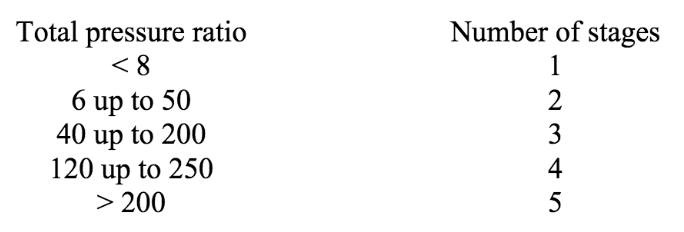
\includegraphics[scale=0.8]{ch5/22}
\captionof{table}{}
\end{center}

We can see that some pressure ratios are situated in 2 stage numbers. One has to choose in function of the use. If we use the compressor everyday continuously, then it is better to invest more at the acquisition to lower the maintenance and consumption costs. If we use it for example once a day, then take the cheapest. 

\section{Centrifugal turbochargers}
\subsection{Introduction}

\minifig{ch5/23}{ch5/24}{0.3}{0.3}{0.49}{0.49}
This is one of the most efficient compression system for high compression ratio. The wheel is mounted on the shaft and on this wheel we have a passage for the flow between blades. On top of that we have a cover. The blades can be purely radial or shifted. Then we enter in the diffuser where we have vanes (2 rows), before going into the volute. This collector can have different shapes. The volume is increasing as shown on the second figure, it is used mainly to change the direction of the air. The distributor is different from the pump because we have something inside, we have vanes in the distributor. These vanes can rotate in some cases. They are called Variable Stator Vane, or Inlet Guide Vane.
